\subsection{Aircrafts screens}\label{subsec:aircrafts-screens}
\textbf{Aircrafts screen} (Figure \ref{fig:aircrafts}) contains a list of added aircrafts.
In addition, a user can add a new drone view Add button.
A user will get to this screen from Profile screen after the click to the My Aircrafts button.

\textbf{Aircraft screen} (Figure \ref{fig:new_aircraft}) is for display the detail of an aircraft.
Simultaneously, it is used for adding new aircraft.
A user will get to it after choose a one from the list in \textbf{Aircrafts screen}.
This screen contains a form with four text fields:
\begin{itemize}
    \item the first is for type name,
    \item the second is for type UAS Operator ID what identify a person that has permitions to flight with drones and passed the pilot exams,
    \item the third and four is for choosing the vendor and its model, and
    \item the last one is for setting the weight of aircraft
\end{itemize}


\begin{figure}
    \centering
    \begin{minipage}{.45\textwidth}
        \centering
        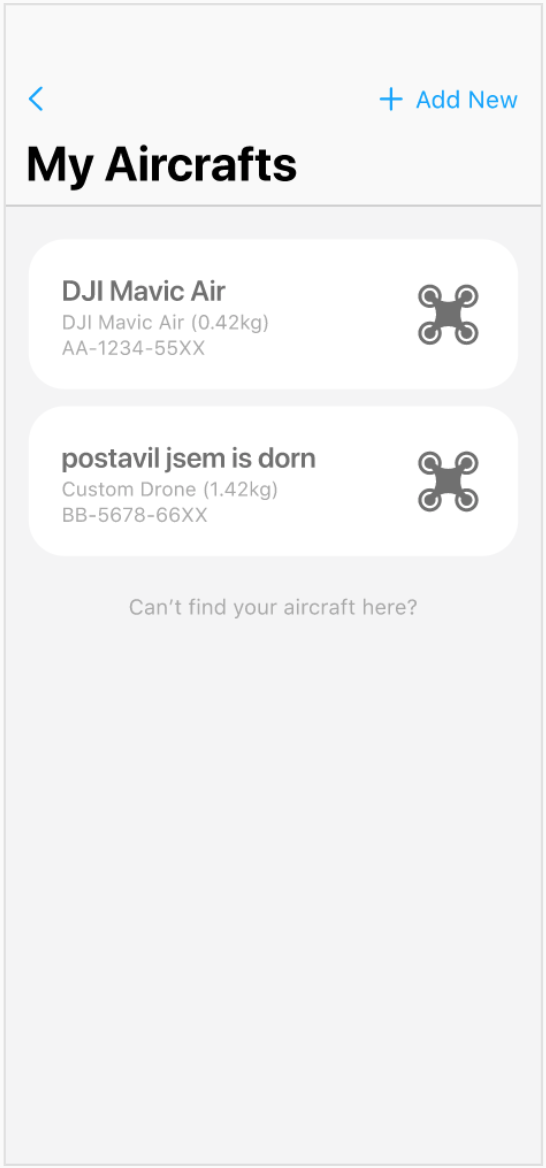
\includegraphics[width=.7\linewidth]{assets/user_interface_design/aircraft/aircrafts.png}
        \caption{[A24] Aircrafts}
        \label{fig:aircrafts}
    \end{minipage}%
    \hspace{.05\linewidth}
    \begin{minipage}{.45\textwidth}
        \centering
        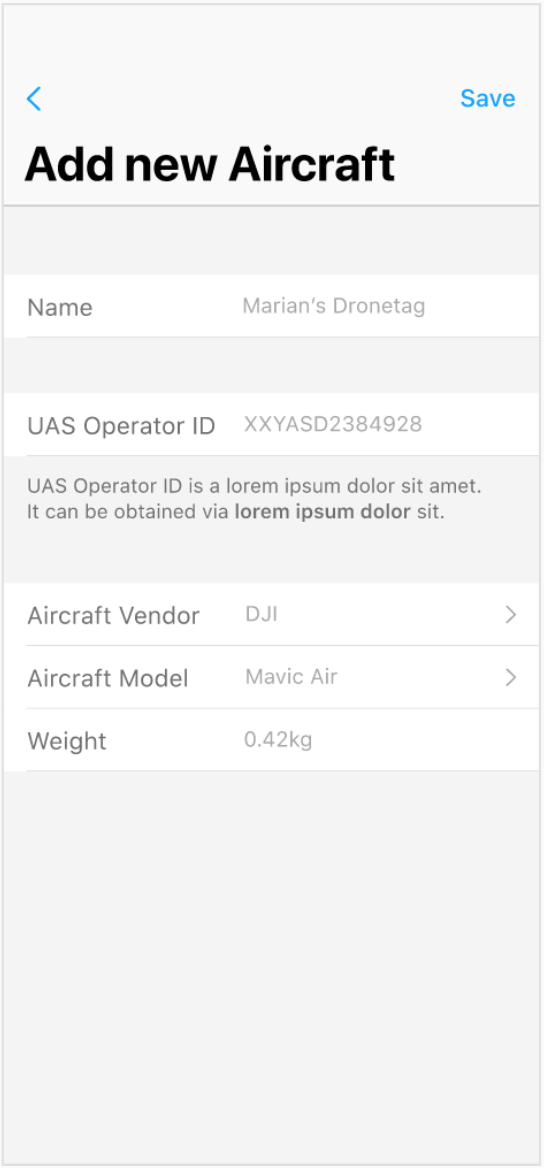
\includegraphics[width=.7\linewidth]{assets/user_interface_design/aircraft/new_aircraft.png}
        \caption{[A25] New Aircraft}
        \label{fig:new_aircraft}
    \end{minipage}
    \label{fig:aircrafts_all}
\end{figure}
